\documentclass[20pt]{extarticle}
\usepackage[papersize={41in, 36in}]{geometry}
\usepackage[poster]{tcolorbox}
\usepackage{graphicx}
\usepackage{natbib}
\usepackage[T1]{fontenc}
\usepackage{hyperref}
\usepackage[sfdefault]{FiraSans}
\renewcommand*\oldstylenums[1]{{\firaoldstyle #1}}
\renewcommand{\bibsection}{}

\definecolor{col1}{HTML}{99a5b8}
\definecolor{col2}{HTML}{003049}

\pagestyle{empty}
\begin{document}
\begin{tcbposter}[
  coverage = {
    spread,
    interior style = {color=col2}
  },
  poster = {columns=4,rows=5, spacing=5mm},
  boxes = {
    enhanced standard jigsaw,
    fonttitle=\bfseries\LARGE,
    arc=20px,
    boxrule=2mm,
    colframe=col1,
    colback=white,
    opacityback=1.0,
    title style = {color=col1}
  }
  ]
  % Here, we insert the poster content later

  \posterbox[height=2.4in, underlay={
    \node[right,inner sep=0pt,outer sep=0.5in] at (frame.west) {
\includegraphics[height=2in]{columbia.pdf}};
    \node[left,inner sep=0pt,outer sep=0.5in] at (frame.east) {
\includegraphics[height=2in]{THEA_logo.png}};
  }]{name=title, column=1, span=4, below=top}{
    \begin{center}
      \vspace{20px}\resizebox{34in}{!}{\Huge\bfseries Simulating magnetic field amplification by the Kelvin-Helmholtz dynamo in neutron star mergers}\\[3mm]
      {\LARGE Benjamin Goldman, Columbia University Physics Department} \hspace{1in} {\LARGE Simulation codes avaliable at \url{https://github.com/ben-goldman/khmhd}}
    \end{center}
  }
  \posterbox[adjusted title=Background]{name=background, column=1, span=2, below=title}{
    \begin{description}
      \item[Neutron Star (NS):] Extremely dense core of collapsed massive stars
      \item[Instability:] System in which perturbations grow exponentially
      \item[Turbulence:] Disorderly fluid state characterized by vortex motion and energy dissipation
      \item[Dynamo:] Self-sustaining process where turbulence within a conducting fluid amplifies an existing magnetic field
    \end{description}
  }
  \posterbox[adjusted title=Neutron Star Mergers]{name=nsmergers, column=1, span=2, below=background}{
    \begin{itemize}
      \item Gravitational waves emitted during inspiral as stars spiral in.
      \item {\bfseries Short-lived coalescense phase in which stars merge.}
      \item Particles and gamma rays are emitted during accretion as energy is released.
      \item Lower-energy waves continue to be emitted from collision remnant.
    \end{itemize}
    \begin{center}
      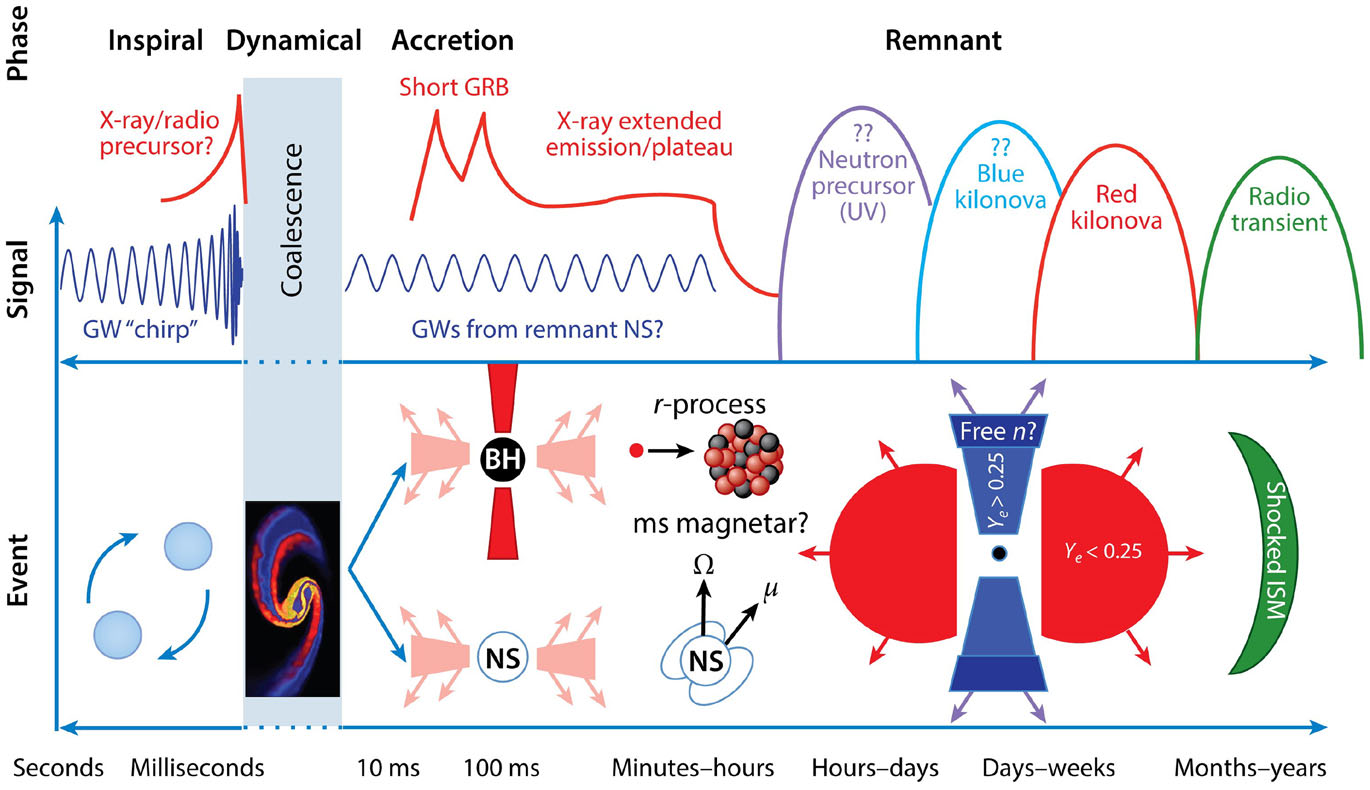
\includegraphics[width=0.8\textwidth]{timeline.png} \\
      {\bfseries Figure 1.} Summary of the phases of a neutron star collision \citep{burns2020a}
    \end{center}
  }
  \posterbox[adjusted title=Background research]{name=background, column=1, span=2, below=nsmergers}{
    \begin{itemize}
      \item \citet{palenzuela2022} applied GRMHD (general relativity magnetohydrodynamics) to simulate coalescence phase of neutron star collision.
      \item Magnetic field amplified in Kelvin-Helmholtz instability in core of merging system.
      \item Required to mathematically approximate dynamo, rather than simulate turbulent flow due to immense computational complexity of simulation.
    \end{itemize}
    \begin{center}
      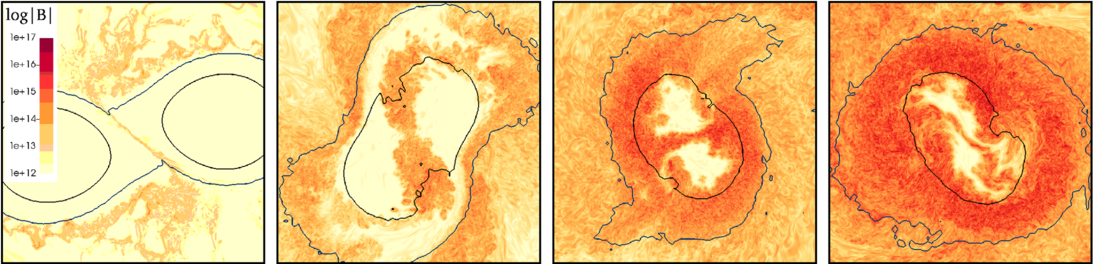
\includegraphics[width=0.9\textwidth]{merger.png} \\
      {\bfseries Figure 2.} Magnetic field development in GRMHD neutron star merger simulation \citep{palenzuela2022}
    \end{center}
  }
  \posterbox[adjusted title=The Kelvin-Helmholtz instability]{name=kelvinhelmholtz, column=1, span=2, below=background}{
    \begin{itemize}
      \item Opposing fluid velocity layer produces unstable system.
      \item Initially when perturbed, wavelike "lumps" develop.
      \item Eventually becomes turbulent as waves grow and interact.
    \end{itemize}
    \begin{center}
      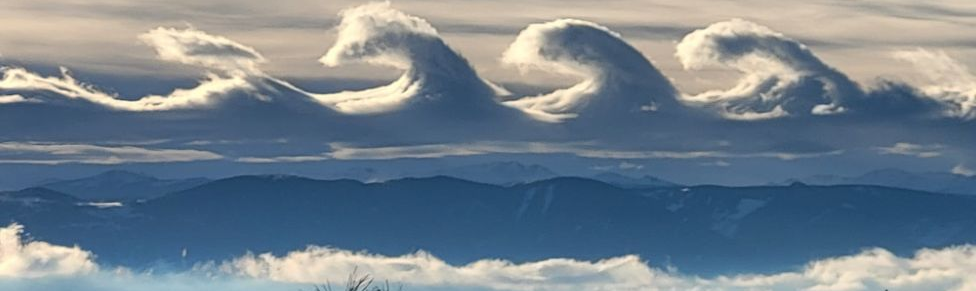
\includegraphics[width=0.9\textwidth]{clouds.png}\\
      {\bfseries Figure 3.} Clouds formed by the Kelvin-Helmholtz instability in the Earth's atmosphere (Rachel Gordon/BBC)
    \end{center}
  }
  \posterbox[adjusted title=Methods]{name=methods, column=3, span=2, below=title}{
    \begin{itemize}
      \item Used spectral MHD solver SpectralDNS \citep{mortensen2016} to simulate the Kelvin Helmholtz insatability on Columbia Ginsburg cluster.
      \item Initialized model with weak magnetic field and small velocity perturbations.
      \item Ran simulation until magnetic field stabilized.
      \item Recorded magnetic energy spectrum and growth rate.
    \end{itemize}
  }
  \posterbox[adjusted title=Results]{name=results, column=3, span=2, below=methods}{
    \begin{center}
      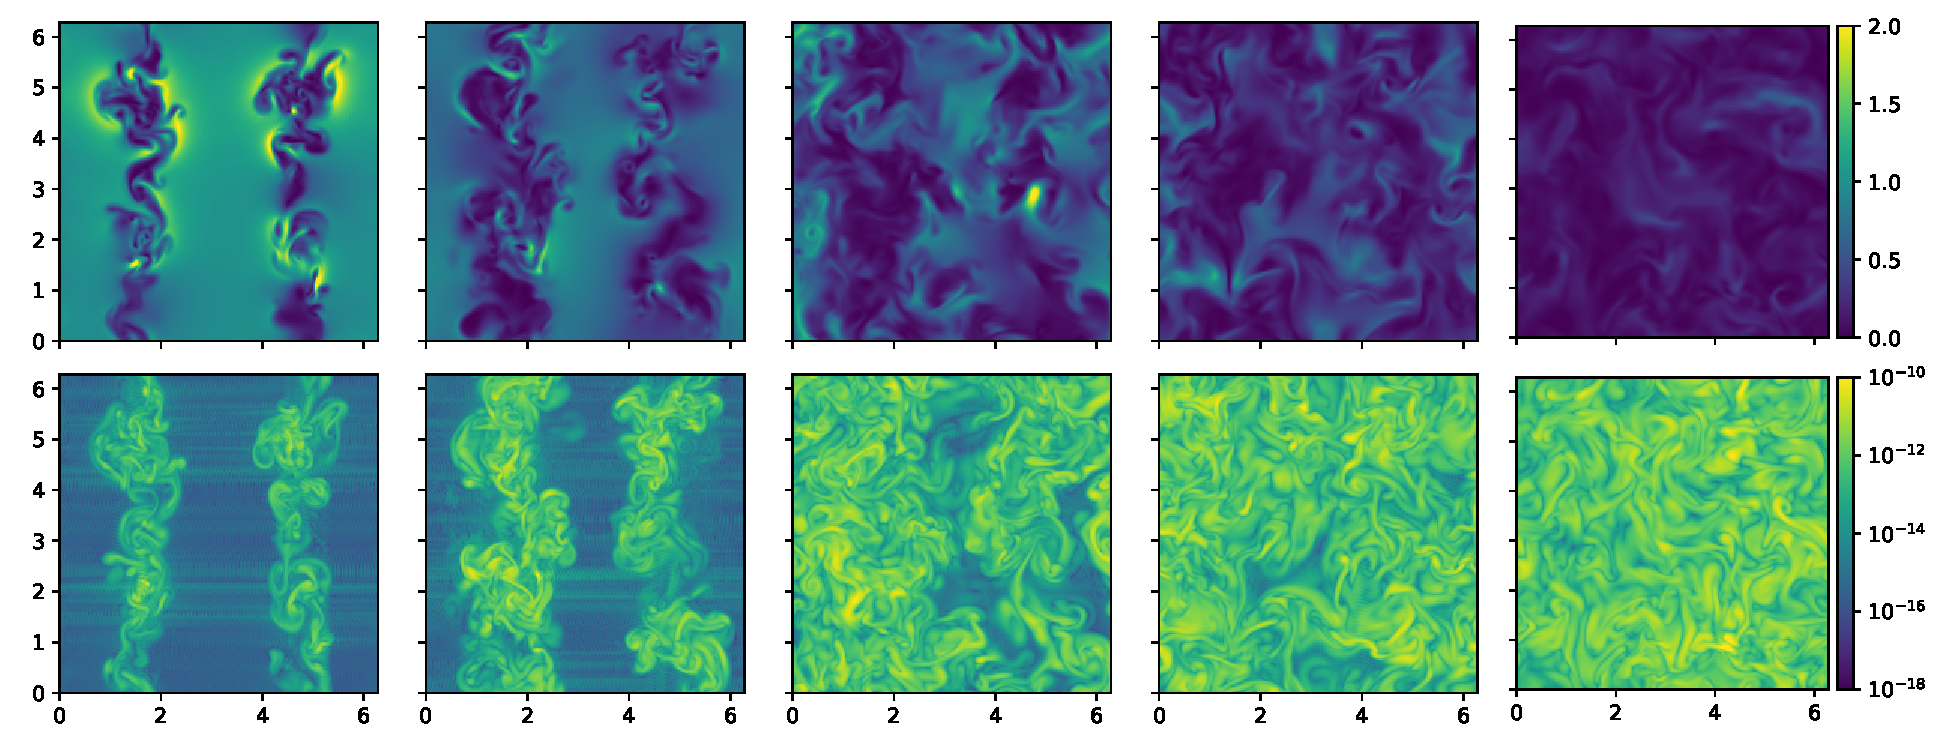
\includegraphics[width=0.8\textwidth]{images.pdf} \\
      {\bfseries Figure 4.} Kinetic (top) and magnetic (bottom) field strength at selected timesteps.
    \end{center}
    \begin{itemize}
      \item 3-dimensional waves and eddies develop before turbulence onset.
      \item Magnetic field grows first during wavelike KH growth phase and then again during early development of turbulence.
      \item Kinetic energy dissipates during turbulence while magnetic field stays stable.
      \item Dynamo efficiency dependent on fluid velocity, i.e., dies down as turbulence dissipates.
    \end{itemize}
    \begin{center}
      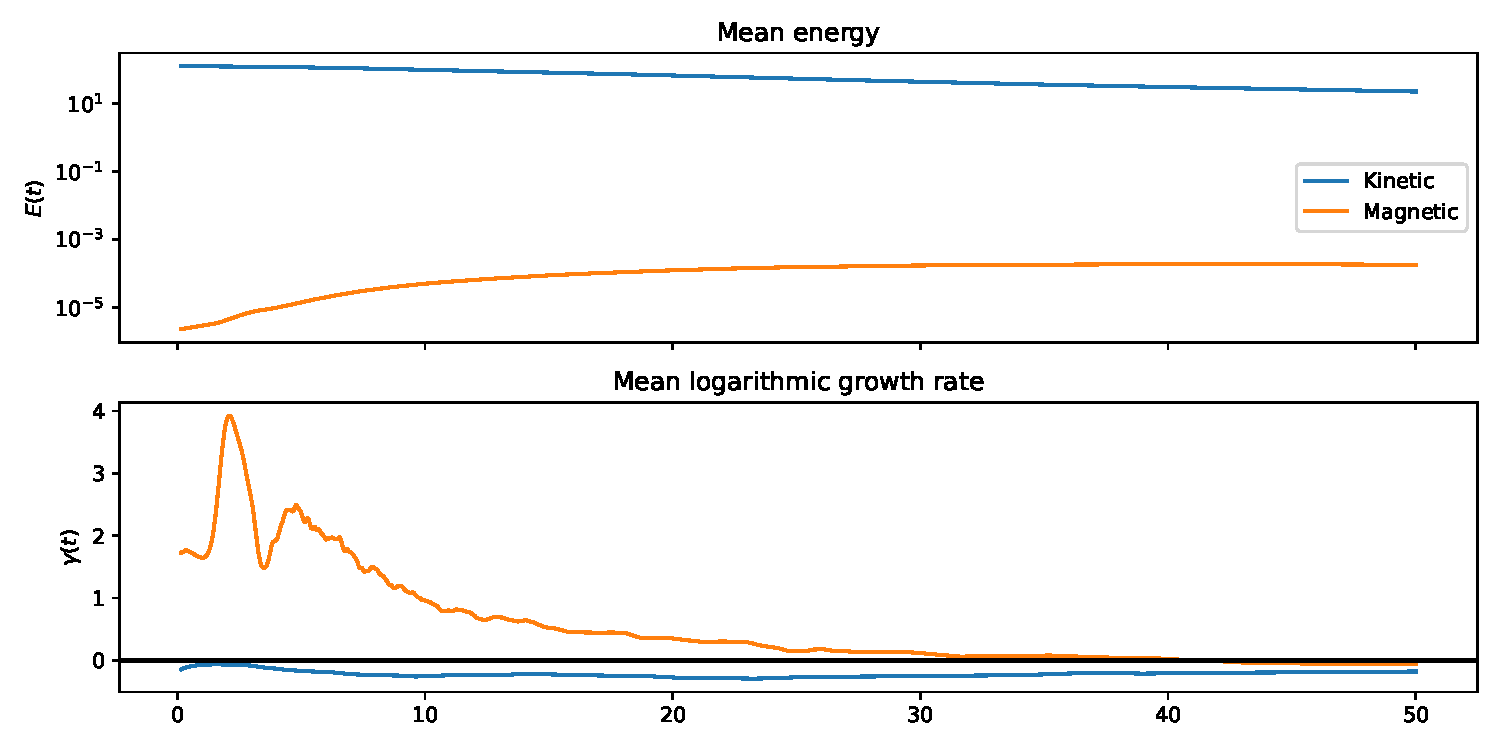
\includegraphics[width=0.8\textwidth]{lines.pdf} \\
      {\bfseries Figure 5.} Kinetic and magnetic mean energy and logarithmic field growth rate.
    \end{center}
  }
  \posterbox[adjusted title=Conclusions]{name=conclusions, column=3, span=2, below=results}{
    \begin{itemize}
      \item Successfully simulated MHD system with realistic initial conditions.
      \item The Kelvin Helmholtz instability can produce an efficient dynamo.
      \item Magnetic field is amplified mostly during early coalescence.
    \end{itemize}
  }
  \posterbox[adjusted title=Next steps]{name=nextsteps, column=3, span=2, below=conclusions}{
    \begin{itemize}
      \item Rerun simulations under different choices of Reynolds number/viscosity
      \item Introduce angular momentum of neutron stars.
      \item Calculate relationship between maximum dynamo growth rate and Reynolds number to produce theoretical model.
      \item Combine results with large-scale understanding towards a theory of GRB origin.
    \end{itemize}
  }
  \posterbox[adjusted title=References]{name=references, column=3, span=2, below=nextsteps}{
    \nocite{burns2020a}
    \bibliographystyle{apalike}
    \bibliography{refs.bib}
  }
  \posterbox[adjusted title=Acknowledgements]{name=acknowledgements, column=3, span=2, below=references}{
    \begin{itemize}
      \item Valentin Skoutnev, my research mentor
      \item The Laidlaw Foundation and the Columbia Undergraduate Research and Fellowships office
    \end{itemize}
  }
\end{tcbposter}

\end{document}
